\chapter{What the Book Missed}\label{chap:missed}

This chapter goes back over the two halves of the conjecture and asks whether anything within reach was left on the table. Two things were.

On the cycle side, the basic inequality of \cref{chap:cycles} bounds the smallest element $M$ of a cycle with $r$ odd elements by $F(r)=r/(3\Lambda)$. We show that the right constant is not $1$ but $1/(2\log 2)\approx 0.7213$, uniformly in the word, and that this constant cannot be improved by any argument that sees only $r$, the number of halvings $s$ and the minimum: positive rational cycles attain it. The improvement beats both the run bound of \cref{ex:ch20:run} and the constant $3/4$ of Hercher's Theorem~27~\cite{hercher2023}. Its real value is diagnostic. It says exactly how much of the current record is arithmetic: to exclude the rung $r^\ast=72\,057\,431\,991$ from verification to $2^{71}$, a proof must extract a factor of at least $1.33$ from the integrality of the cycle, and no inequality in $(r,s,M)$ alone will ever do it. The inequality is the shadow of an exact identity, $3M(2^{\delta_c}-1)=\sum_t2^{W_t}$ over the walk of halvings read from the minimum, and the identity says what the word of a cycle above the verification range must look like: for a cycle at $r^\ast$ with minimum above $2^{71}$ the halving count stays within three of $t\log_23$ nearly half of the time. A uniformly random admissible word does nothing of the kind.

On the divergence side, the frequency criterion of \cref{chap:divergence} (\cref{cor:ch9:freq}) can be rewritten as a statement about the empirical measures of an orbit on the 2 adic integers, and then truncated. The result is a finite modulus target: an orbit is bounded as soon as the odd iterates in the classes $1$ and $5$ modulo $8$, with class $5$ counted twice, have lower frequency above $\log_2(3/2)\approx 0.585$. Equidistribution would give $0.75$.

Neither result proves anything about the conjecture. Both sharpen the description of what a proof has to do, and both come with a computation that can be run.

\section{Where the two halves stand}\label{sec:ch20:stand}

\Cref{chap:path} split the conjecture into a cycle half and a divergence half. After \cref{chap:cycles} to \cref{chap:backward} the position is as follows.

\paragraph{Cycles.} A nontrivial cycle has $r\ge 72\,057\,431\,991$ odd elements by the method of \cref{chap:cycles} with verification to $2^{68}$, and $r\ge 137\,528\,045\,312$ by Hercher's residue computation~\cite{hercher2023} with verification to $3\cdot 2^{69}$ (made unconditional by Ba\v{r}ina's verification to $2^{71}$~\cite{barina2025}). Both numbers come from one inequality,
\begin{equation}\label{eq:ch20:cycleid}
\Lambda:=s\log 2-r\log 3=\sum_{t=0}^{r-1}\log\Bigl(1+\frac{1}{3x_t}\Bigr)<\sum_{t=0}^{r-1}\frac{1}{3x_t},
\end{equation}
the cycle identity of \cref{sec:ch8:identity}, together with a lower bound on the elements $x_t$. \Cref{chap:cycles} uses $x_t\ge M$ for every $t$. That is the step we revisit.

\paragraph{Divergence.} An orbit is unbounded only if the running mean $\bar k_N$ of the halving exponents has upper limit at most $\log_2 3$ (\cref{cor:ch9:freq}). No method controls $\bar k_N$ along a single orbit.

\section{The minimum inequality made sharp}\label{sec:ch20:sharp}

Fix a cycle of the Syracuse map, integer or rational, with odd elements $x_0,\dots,x_{r-1}$ and halving exponents $k_0,\dots,k_{r-1}$, so that $x_{t+1}=(3x_t+1)/2^{k_t}$ with indices modulo $r$. Write
\[
\theta=\log_2 3,\qquad s=\sum_t k_t,\qquad K_t=k_0+\dots+k_{t-1}\ (K_0=0),\qquad W_t=K_t-t\theta .
\]
$W$ is the walk of halvings against its expected slope; it starts at $W_0=0$ and ends at $W_r=s-r\theta=\Lambda/\log 2$, which is positive for every cycle by \eqref{eq:ch20:cycleid}. Iterating the map gives the product formula
\begin{equation}\label{eq:ch20:product}
x_t=x_0\,2^{-W_t}\prod_{j<t}\Bigl(1+\frac{1}{3x_j}\Bigr),\qquad 0\le t\le r .
\end{equation}

\begin{lemma}[The walk seen from the extremes]\label{lem:ch20:walk}
Let $\delta_c=s-r\theta=W_r$.
\begin{enumerate}[label=(\roman*)]
\item If $x_0=M$ is the smallest element, then $W_t\le\delta_c$ for $0\le t\le r$, and so $K_t\le\lfloor t\theta+\delta_c\rfloor$.
\item If $x_0=N$ is the largest element, then $W_t\ge 0$ for $0\le t\le r$, and so $K_t\ge\lceil t\theta\rceil$.
\end{enumerate}
\end{lemma}

\begin{proof}
The product in \eqref{eq:ch20:product} lies between $1$ and the full product $\prod_{j<r}(1+1/(3x_j))=2^s/3^r=2^{\delta_c}$. In (i), $x_t\ge M=x_0$ gives $2^{W_t}\le\prod_{j<t}(1+1/(3x_j))\le 2^{\delta_c}$. In (ii), $x_t\le N=x_0$ gives $2^{W_t}\ge\prod_{j<t}(1+1/(3x_j))\ge 1$. The statements about $K_t$ follow because $K_t$ is an integer.
\end{proof}

Part (i) is the precise form of the observation that the minimum of a cycle has infinite stopping time: from the minimum, the halvings never get ahead of the line $t\theta$ by more than the closing defect $\delta_c$. Part (ii) is its mirror. Neither uses integrality.

The cycle formula of \cref{sec:ch8:identity}, summed along the cycle, gives an exact identity that the rest of the section only estimates.

\begin{theorem}[Exact form of the cycle identity]\label{thm:ch20:exact}
For every positive rational cycle and every choice of the starting element $x_0$,
\begin{equation}\label{eq:ch20:exact}
3x_0\bigl(2^{\delta_c}-1\bigr)=\Phi(w):=\sum_{t=0}^{r-1}2^{W_t},
\end{equation}
where $W_t=K_t-t\theta$ is the walk of the word read from $x_0$.
\end{theorem}

\begin{proof}
Iterating $2^{k_t}x_{t+1}=3x_t+1$ around the cycle gives $2^sx_0=3^rx_0+\sum_{j<r}3^{r-1-j}2^{K_j}$, so $x_0(2^s-3^r)=3^{r-1}\sum_j2^{K_j}3^{-j}=3^{r-1}\sum_j2^{W_j}$. Divide by $3^r$.
\end{proof}

Since $2^{\delta_c}-1=e^{\Lambda}-1\ge\Lambda$, \eqref{eq:ch20:exact} gives $3x_0\Lambda\le\Phi(w)$ from any starting point, with a loss of only a factor $e^{\Lambda}$. From the minimum, \cref{lem:ch20:walk}(i) caps each term.

\begin{theorem}[Sharp minimum inequality]\label{thm:ch20:min}
For every positive rational cycle with $r$ odd elements, $s$ halvings and smallest element $M$,
\begin{equation}\label{eq:ch20:min}
3M\Lambda<B_r(\delta_c):=\sum_{t=0}^{r-1}\min\bigl\{1,\;2^{\lfloor t\theta+\delta_c\rfloor-t\theta}\bigr\},\qquad\delta_c=s-r\theta .
\end{equation}
\end{theorem}

\begin{proof}
Rotate so that $x_0=M$. By \eqref{eq:ch20:product}, $x_t\ge M\,2^{-W_t}$, and $x_t\ge M$. Hence $1/x_t\le M^{-1}\min\{1,2^{W_t}\}$, and $W_t=K_t-t\theta\le\lfloor t\theta+\delta_c\rfloor-t\theta$ by \cref{lem:ch20:walk}(i). Insert this in \eqref{eq:ch20:cycleid}. (Equivalently, apply the cap to \eqref{eq:ch20:exact}; the two routes differ by the factor $e^{\Lambda}$ and by $2^{\delta_c}$ against $1$ in the cap.)
\end{proof}

The right side of \eqref{eq:ch20:min} depends only on $r$ and $\delta_c$, not on the word. When $\{t\theta\}+\delta_c<1$ the $t$th term is $2^{-\{t\theta\}}$; otherwise it is at most $1$. Write $\delta(t)=\lceil t\theta\rceil-t\theta$ as in \cref{chap:cycles}, so that the exceptional $t$ are those with $\delta(t)\le\delta_c$.

\begin{corollary}[On the ladder]\label{cor:ch20:ladder}
Let $r$ be a rung of the ladder of \cref{chap:cycles}, that is $\delta(t)>\delta(r)$ for $1\le t<r$, and put
\[
B_r=\sum_{t=0}^{r-1}2^{-\{t\theta\}},\qquad G(r)=\frac{B_r}{3\log 2\;\delta(r)} .
\]
Then every cycle with $r$ odd elements has $M<G(r)$. For every $r$, $B_r=r/(2\log 2)+O\bigl(\sum_{i\le k+1}a_i\bigr)$, where $a_i$ are the partial quotients of $\theta$ and $q_k\le r<q_{k+1}$.
\end{corollary}

\begin{proof}
A cycle with $s=\lceil r\theta\rceil$ has $\delta_c=\delta(r)$ and $\Lambda=\delta(r)\log 2$; at a rung no $t<r$ is exceptional, so $B_r(\delta_c)=B_r$. A cycle with $s=\lceil r\theta\rceil+j$, $j\ge1$, has $\Lambda\ge(\delta(r)+j)\log2$ and $B_r(\delta_c)\le r$, so its bound $r/(3\log2\,(\delta(r)+j))$ is below $G(r)$ because $B_r>r/2$ and $\delta(r)<1$. The asymptotic is Koksma's inequality for the function $u\mapsto 2^{-u}$, of variation $1/2$ on $[0,1)$, combined with Ostrowski's bound on the discrepancy of $\{t\theta\}$ in terms of the partial quotients \cite[Chapter~2]{kuipers1974}.
\end{proof}

Since $\int_0^1 2^{-u}\,du=1/(2\log 2)$, the corollary says that $M<\bigl(1/(2\log2)+o(1)\bigr)F(r)$ with $F(r)=r/(3\log 2\,\delta(r))$ the bound of \cref{chap:cycles}. Three earlier constants sit above it:
\begin{itemize}
\item the crude bound $x_t\ge M$, constant $1$;
\item the run bound from an independent review of the first edition, $M<(r+s)/(9\Lambda)$, constant $(1+\theta)/3\approx0.862$ (\cref{ex:ch20:run});
\item Hercher's Theorem~27, which bounds the average reciprocal by $3/(4X_0)$, constant $3/4$.
\end{itemize}
The constant is $1/(2\log2)=0.72135$. \Cref{fig:ch20:cycle}(b) shows $B_r/r$ along the rungs: it equals $1$ at $r=1$, falls below $3/4$ at $r=17$, and is $0.72135$ to five digits from $r=10^7$ on. We computed $B_r$ exactly up to $2\cdot10^7$ and, for the large rungs, by binning the fractional parts $\{t\theta\}$ in exact $128$ bit fixed point arithmetic, which brackets $B_{r}$ to a relative width of $10^{-5}$ (script \texttt{br\_sum.c}, in \texttt{scripts/ch20/code} with the other scripts of this chapter). The bracket is a proof up to the truncation of $\theta$ to $128$ bits: the function $u\mapsto2^{-u}$ is monotone on each bin, so the two bin sums enclose the sum over the computed fractional parts, and these differ from the true ones by less than $t\,2^{-128}<2^{-92}$, which moves a point to another bin only if it lies that close to one of the $2^{16}$ bin edges; below $r^\ast$ the expected number of such points is about $2^{-39}$. At $r^\ast=72\,057\,431\,991$ the bracket is $[51\,978\,175\,019,\ 51\,978\,724\,775]$ and $r^\ast/(2\log2)=51\,978\,449\,896$ lies inside it.

\section{Rational cycles meet the bound}\label{sec:ch20:ratl}

Every finite word $(k_0,\dots,k_{r-1})$ with $2^s>3^r$ determines exactly one positive rational cycle (of period $r$, or of a divisor of $r$ when the word is a power of a shorter word), whose element $x_0=c/(2^s-3^r)$ with $c=\sum_j3^{r-1-j}2^{K_j}$ is the 2 adic point of the periodic parity sequence (\cref{sec:ch8:rational} and \cref{ex:ch20:rational}). Everything in \cref{sec:ch20:sharp} applies to these cycles. The following theorem shows that \eqref{eq:ch20:min} is attained by them, so no inequality that uses only $r$, $s$ and $M$ can improve the constant.

\begin{theorem}[Christoffel cycles are extremal]\label{thm:ch20:christoffel}
Let $s/r>\theta$ be in lowest terms, $\delta=s-r\theta$, and let $w$ be the lower Christoffel word of slope $s/r$, defined by $K_t=\lfloor ts/r\rfloor$. The rational cycle of $w$ has smallest element $M_w$ with
\begin{equation}\label{eq:ch20:christ}
2^{-2\delta}\,\beta_r\;\le\;3M_w\Lambda\;<\;B_r(\delta),
\end{equation}
where
\[
\beta_r=\sum_{j=0}^{r-1}2^{-j/r}=\frac{1}{2(1-2^{-1/r})}=\frac{r}{2\log2}+\frac14+O(1/r).
\]
In particular, along the rungs of the ladder, $3M_w\Lambda/B_r\to1$ and $M_w/F(r)\to1/(2\log2)$.
\end{theorem}

\begin{proof}
Put $a_t=2^{K_t}/3^t=2^{W_t}$. Since $K_t=ts/r-\{ts/r\}$, we have $W_t=t\delta/r-\{ts/r\}$, so $2^{-\{ts/r\}}\le a_t\le2^{\delta}$. Summing the cycle formula gives $x_0=\sum_ja_j/(3(2^\delta-1))$, and $2^\delta-1\le\delta\log2\cdot2^\delta=\Lambda2^\delta$. As $t$ runs over $0,\dots,r-1$ the residues $ts\bmod r$ run over $0,\dots,r-1$, so $\sum_ja_j\ge\sum_j2^{-\{js/r\}}=\beta_r$, and $x_0\ge\beta_r/(3\Lambda2^\delta)$. Finally \eqref{eq:ch20:product} gives $x_t\ge x_02^{-W_t}\ge x_02^{-\delta}$ for every $t$, so $M_w\ge x_02^{-\delta}$. This is the left inequality; the right one is \cref{thm:ch20:min}. The expansion of $\beta_r$ is $1/(1-e^{-x})=1/x+1/2+O(x)$ at $x=(\log2)/r$. Along the rungs $\delta\to0$ and $B_r/r\to1/(2\log2)$ by \cref{cor:ch20:ladder}, so both bounds in \eqref{eq:ch20:christ} are $r/(2\log2)\,(1+o(1))$.
\end{proof}

Halbeisen and Hungerb\"uhler~\cite{halbeisen1997} determine the largest minimal element of a rational cycle with a given length and number of odd steps, and show that the cycle of the mechanical word attains it. So the exact bound $B_r/(3(2^{\delta}-1))$ at a rung and its attainment by the Christoffel cycle (\cref{rrt:thm:exact}) are theirs, in another notation (\cref{rrt:rem:hh}). What they do not state is its size: their explicit bound is $\tfrac32F(r)$ near a rung, and the asymptotic constant $1/(2\log2)$ of \cref{cor:ch20:ladder} is not in their paper.

\Cref{tab:ch20:christ} shows how fast the ratio approaches $1$. \Cref{fig:ch20:cycle}(a) shows why: in the Christoffel cycle $\log_2(x_t/M)$ is, up to the tiny drift $t\delta/r$, the fractional part $\{ts/r\}$, so the elements fill the interval $[M,2M]$ evenly in logarithmic scale. That is the most reciprocal mass a cycle can carry given its minimum.

\begin{table}[t]
\centering
\begin{tabular}{rrcccc}
\toprule
$r$ & $s$ & $M_w/F(r)$ & $3M_w\Lambda/B_r$ & $N_w/F(r)$ & $B_r/r$\\
\midrule
1 & 2 & 0.863046 & 0.863046 & 0.86305 & 1.000000\\
5 & 8 & 0.767308 & 0.974168 & 1.33978 & 0.787654\\
41 & 65 & 0.727312 & 0.994279 & 1.43037 & 0.731497\\
306 & 485 & 0.722162 & 0.999489 & 1.44106 & 0.722532\\
15\,601 & 24\,727 & 0.721364 & 0.999991 & 1.44266 & 0.721370\\
190\,537 & 301\,994 & 0.721349 & 1.000000 & 1.44269 & 0.721349\\
10\,781\,274 & 17\,087\,915 & 0.721348 & 1.000000 & 1.44269 & 0.721348\\
\midrule
\multicolumn{2}{r}{limit} & $1/(2\log2)$ & $1$ & $1/\log2$ & $1/(2\log2)$\\
\bottomrule
\end{tabular}
\caption{The rational cycles of the Christoffel words at rungs of the ladder. $M_w$ and $N_w$ are the smallest and largest elements, $F(r)=r/(3\Lambda)$. The ratio $3M_w\Lambda/B_r$ is the fraction of the bound of \cref{thm:ch20:min} that the cycle attains. The trivial cycle $r=1$ is the Christoffel cycle of slope $2$. Script \texttt{sharp.py}.}
\label{tab:ch20:christ}
\end{table}

\begin{figure}[t]
\centering
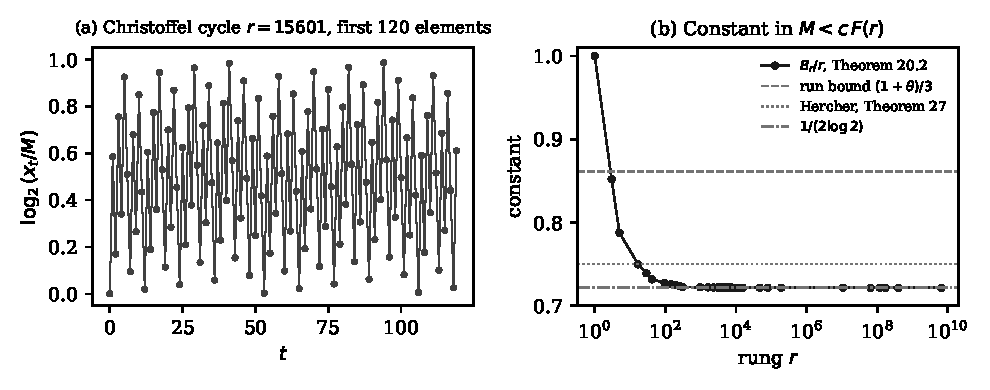
\includegraphics[width=\textwidth]{figures/ch20_cycle.pdf}
\caption{(a) The first $120$ odd elements of the Christoffel rational cycle with $r=15\,601$, $s=24\,727$, on the scale $\log_2(x_t/M)$. They follow the fractional parts $\{ts/r\}$ and fill $[M,2M]$ evenly. (b) The constant $c$ in $M<c\,F(r)$ along the rungs: $B_r/r$ from \cref{thm:ch20:min}, the run bound $(1+\theta)/3$, Hercher's $3/4$, and the limit $1/(2\log 2)$.}
\label{fig:ch20:cycle}
\end{figure}

\section{The largest element}\label{sec:ch20:max}

The same argument, run from the top, bounds the largest element from below.

\begin{theorem}[Sharp maximum inequality]\label{thm:ch20:max}
For every positive rational cycle with $r$ odd elements, smallest element $M$ and largest element $N$,
\[
3N\Lambda\;\ge\;\frac{e^{-\Lambda}}{1+1/(3M)}\,\bigl(2B_r-1\bigr).
\]
\end{theorem}

\begin{proof}
Rotate so that $x_0=N$. By \cref{lem:ch20:walk}(ii), $K_t\ge\lceil t\theta\rceil$, so for $t\ge1$, \eqref{eq:ch20:product} gives $x_t\le N\,2^{t\theta-\lceil t\theta\rceil}e^{\Lambda}=N e^{\Lambda}2^{\{t\theta\}-1}$, the product being at most its full value $e^\Lambda$. Using $\log(1+v)\ge v/(1+v)$ and $3x_t+1\le3x_t(1+1/(3M))$,
\[
\Lambda\ge\sum_t\frac{1}{3x_t+1}\ge\frac{1}{1+1/(3M)}\sum_t\frac{1}{3x_t}\ge\frac{e^{-\Lambda}}{3N(1+1/(3M))}\Bigl(1+\sum_{t=1}^{r-1}2^{1-\{t\theta\}}\Bigr),
\]
and the bracket is $2B_r-1$.
\end{proof}

So the largest element of a long cycle is at least $(1/\log2+o(1))\,F(r)\approx1.4427\,F(r)$, and \cref{tab:ch20:christ} shows that the Christoffel cycles attain this too. Dividing the two theorems gives a statement about shape.

\begin{corollary}[Spread]\label{cor:ch20:spread}
For a cycle at a rung $r$ with $s=\lceil r\theta\rceil$, $N/M>e^{-\Lambda}(2B_r-1)/\bigl((1+1/(3M))B_r\bigr)$. For long cycles of integers this is $2-o(1)$: the elements of any long cycle span at least a factor of about two, and the extremal cycles span exactly that.
\end{corollary}

The crude argument gives only the trivial spread $3/2$ from a single step with $k=1$.

\section{What the sharp inequality buys}\label{sec:ch20:buys}

\Cref{tab:ch20:thresh} converts the four inequalities into the verification range at which each rung is excluded. \Cref{thm:ch20:min} lowers every threshold of \cref{tab:ch8:thresholds} by about $\log_2(2\log2)=0.4712$ (the limit along the rungs; $0.4689$ at $r=306$), against $0.2148$ for the run bound and $0.4150$ for Hercher's Theorem~27.

\begin{table}[t]
\centering
\small
\begin{tabular}{rrrrrr}
\toprule
rung $r$ & $\log_2F$ & run bound & Hercher 27 & Thm.~\ref{thm:ch20:min} & $B_r/r$\\
\midrule
306 & 16.6065 & 16.3917 & 16.1914 & 16.1376 & 0.722532\\
15\,601 & 28.0905 & 27.8757 & 27.6755 & 27.6193 & 0.721370\\
190\,537 & 39.8407 & 39.6259 & 39.4257 & 39.3695 & 0.721349\\
10\,781\,274 & 48.0648 & 47.8500 & 47.6497 & 47.5935 & 0.721348\\
397\,573\,379 & 60.1190 & 59.9042 & 59.7040 & 59.6478 & 0.721348\\
6\,586\,818\,670 & 67.5555 & 67.3407 & 67.1405 & 67.0843 & 0.721348\\
72\,057\,431\,991 & 71.8843 & 71.6695 & 71.4693 & 71.4131 & 0.721348\\
137\,528\,045\,312 & 75.4333 & 75.2185 & 75.0182 & 74.9620 & 0.721348\\
\bottomrule
\end{tabular}
\caption{$\log_2$ of the verification range above which a cycle with $r$ odd elements is excluded, at selected rungs, under the crude bound $F(r)$, the run bound $(r+s)/(9\Lambda)$, Hercher's Theorem~27 and \cref{thm:ch20:min}. For the four largest rungs $B_r$ is bracketed to relative width $10^{-5}$, which moves the last column by less than $2\cdot10^{-5}$. Script \texttt{thresholds.py}.}
\label{tab:ch20:thresh}
\end{table}

The table does not move the record. With verification to $2^{71}$ the least surviving $r$ is still $r^\ast=72\,057\,431\,991$, since its threshold $2^{71.413}$ exceeds $2^{71}$. \Cref{thm:ch20:christoffel} turns that observation into a statement about methods.

\begin{corollary}[The arithmetic gap at $r^\ast$]\label{cor:ch20:gap}
There is a positive rational cycle with $r^\ast=72\,057\,431\,991$ odd elements and $s=114\,208\,327\,604$ halvings whose smallest element exceeds $2^{71.41}$. Consequently any proof that no integer cycle has $r^\ast$ odd elements, using verification to $2^{71}$, must use a property of integer cycles that rational cycles lack, and that property must improve \cref{thm:ch20:min} at $r^\ast$ by a factor of at least $2^{0.4131}\approx1.33$.
\end{corollary}

\begin{proof}
Apply \cref{thm:ch20:christoffel} at the rung $r^\ast$: $\delta=7.95\times10^{-12}$, so $2^{-2\delta}\beta_{r^\ast}$ differs from $B_{r^\ast}$ by a relative amount below $10^{-5}$, and $M_w\ge2^{71.4131-0.0001}$. Any inequality valid for all positive rational cycles holds for this one, so it cannot imply $M<2^{71}$ for cycles with $r^\ast$ odd elements; only a property that fails for this rational cycle can.
\end{proof}

Hercher's computation does extract such a property: it tracks residue classes of the cycle elements modulo powers of $2$ and excludes $r^\ast$ already at $1536\cdot2^{60}=2^{70.585}$, a factor of $2^{0.828}\approx1.78$ beyond \cref{thm:ch20:min}. \Cref{cor:ch20:gap} explains why some such computation is unavoidable, and it fixes the scale of the next step. To pass the following rung $q_{23}=137\,528\,045\,312$ from verification to $2^{71}$, a method needs a factor of $2^{3.96}\approx15.6$ beyond \cref{thm:ch20:min}, or verification to $2^{74.96}$. That is the honest measure of the cycle half as it stands: one rung of the ladder costs a factor of about sixteen in either arithmetic or computation.

\section{What the word of a cycle must look like}\label{sec:ch20:band}

\Cref{thm:ch20:exact} says that a cycle with minimum $M$ has $\Phi(w)=3M(2^{\delta_c}-1)$ for the word read from $M$, with $\Phi(w)\le B_r(\delta_c)$. A cycle with $M\ge X$ therefore needs
\begin{equation}\label{eq:ch20:need}
\frac{\Phi(w)}{r}\ \ge\ \frac{3X\Lambda}{r}.
\end{equation}
At $r^\ast$ and $X=2^{71}$ the right side is $0.5417$, against the maximum $B_{r^\ast}/r^\ast=0.7213$. So the walk read from the minimum must keep $2^{W_t}$ at three quarters of the largest average any word allows. How restrictive is that? Call a word \emph{admissible} if $k_t\ge1$, $K_r=s$ and $K_t\le\lfloor t\theta+\delta_c\rfloor$ for all $t$; by \cref{lem:ch20:walk}(i) the word of every cycle read from its minimum is admissible. Admissible words can be counted and sampled exactly by the dynamic programming of \cref{chap:samplers} over the pairs $(t,K_t)$, and \cref{fig:ch20:phi} shows $\Phi(w)/B_r$ for uniform random admissible words at three rungs.

\begin{figure}[t]
\centering
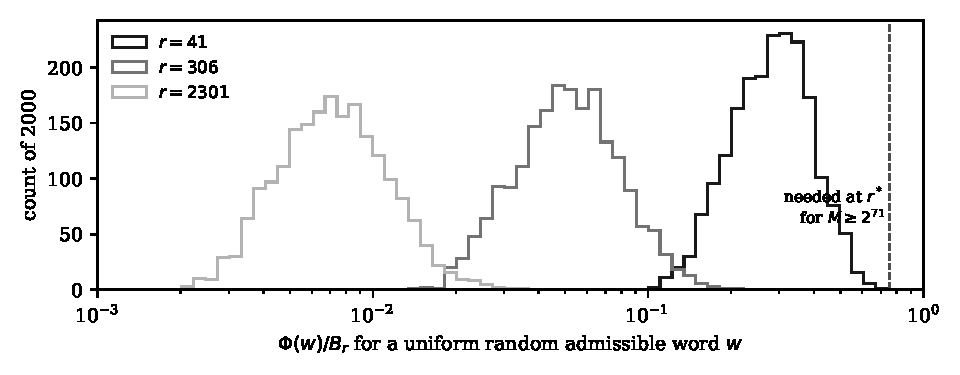
\includegraphics[width=0.9\textwidth]{figures/ch20_phi.pdf}
\caption{The ratio $\Phi(w)/B_r$ for $2000$ uniform random admissible words at the rungs $r=41$, $306$ and $2301$ (script \texttt{admissible.py}). The dashed line is the value \eqref{eq:ch20:need} requires at $r^\ast$ with $X=2^{71}$. A uniform admissible walk wanders far below the line, as a bridge conditioned to stay on one side does, and $\Phi$ stays near a constant: the medians are $0.285$, $0.051$ and $0.0071$, so $\Phi$ itself is about $8.5$, $11$ and $12$.}
\label{fig:ch20:phi}
\end{figure}

A typical admissible word has $\Phi$ of order ten, independent of $r$, and would give a cycle with minimum of order $4/\Lambda$, about $2^{40}$ at $r^\ast$. The words \eqref{eq:ch20:need} allows are the rare ones that stay close to the line, and the next proposition says how close.

\begin{proposition}[Band]\label{prop:ch20:band}
Let a cycle have $r$ odd elements, minimum $M$ and word $w$ read from $M$, and let $b>0$. The fraction $f_b$ of indices $t<r$ with $W_t>-b$ satisfies
\[
f_b\ \ge\ \frac{3M\Lambda/r-2^{-b}}{2^{\delta_c}-2^{-b}} .
\]
At those indices $M\le x_t<2^bMe^{\Lambda}$. In particular a cycle at $r^\ast$ with $M\ge2^{71}$ has $K_t>t\theta-3$, and $x_t<8Me^{\Lambda}$, for at least $47.6$ percent of $t$, and $K_t>t\theta-1$ for at least $8.4$ percent.
\end{proposition}

\begin{proof}
Split \eqref{eq:ch20:exact}: the indices with $W_t>-b$ contribute at most $2^{\delta_c}$ each and the others at most $2^{-b}$ each, so $3M\Lambda\le3M(2^{\delta_c}-1)=\Phi(w)\le r\bigl(f_b2^{\delta_c}+(1-f_b)2^{-b}\bigr)$. The bound on $x_t$ is \eqref{eq:ch20:product} with the product at most $e^{\Lambda}$. The numbers come from $3\cdot2^{71}\Lambda/r^\ast=0.5417$.
\end{proof}

For comparison, the Christoffel word has $W_t\in(-1,\delta_c]$ for every $t$, and a cycle that reached the sharp threshold $2^{71.41}$ would need $f_1\ge0.44$ and $f_3\ge0.68$. So the cycle half at $r^\ast$ is a statement about words whose halving count stays within three of $t\log_23$ half of the time, with half the elements within a factor eight of the minimum, and about no other words. Uniform sampling never produces such a word: among the $2000$ samples at $r=2301$ the largest ratio was $0.036$.

\subsection{Counting the words in the band}

How many admissible words meet the band condition can be computed exactly. Let $N_b(f,r)$ be the number of admissible words of length $r$ (with $s=\lceil r\theta\rceil$) having $W_t>-b$ for at least $fr$ indices. A forward dynamic program over the pairs $(K_t,n_t)$, where $n_t$ counts the indices so far in the band, gives $N_b(f,r)$ for every $f$ at once in $O(r^2s)$ operations (script \texttt{bandcount.py}). \Cref{tab:ch20:band} reports $r^{-1}\log_{10}N_b(f,r)$ at three rungs. The rows stabilise quickly, so the quantity converges to a rate $\rho_b(f)$; the limit of the total is the entropy $\log_{10}\binom{s}{r}/r\to0.4532$, the count of all words with the right number of halvings, because the admissibility constraint costs only a polynomial factor.

\begin{table}[t]
\centering
\small
\setlength{\tabcolsep}{4.5pt}
\begin{tabular}{rrrrrrrrr}
\toprule
& & \multicolumn{3}{c}{$b=1$} & & \multicolumn{3}{c}{$b=3$}\\
\cmidrule{3-5}\cmidrule{7-9}
$r$ & total & $f=0.084$ & $f=0.44$ & $f=0.75$ & & $f=0.476$ & $f=0.68$ & $f=0.75$\\
\midrule
306 & 0.4398 & 0.4268 & 0.3380 & 0.2157 & & 0.4213 & 0.4061 & 0.3992\\
971 & 0.4482 & 0.4327 & 0.3421 & 0.2192 & & 0.4269 & 0.4113 & 0.4041\\
2301 & 0.4509 & 0.4344 & 0.3435 & 0.2204 & & 0.4285 & 0.4128 & 0.4056\\
\bottomrule
\end{tabular}
\caption{$r^{-1}\log_{10}N_b(f,r)$: the exponential rate of the number of admissible words with at least $fr$ indices in the band $W_t>-b$, at three rungs, together with the rate of all admissible words. The pairs $(b,f)$ are those of \cref{prop:ch20:band}: a cycle at $r^\ast$ with $M\ge2^{71}$ needs $(1,0.084)$ and $(3,0.476)$, and one at the sharp threshold needs $(1,0.44)$ and $(3,0.68)$. Script \texttt{bandcount.py}.}
\label{tab:ch20:band}
\end{table}

Two things follow. First, the words that could carry a cycle at $r^\ast$ above $2^{71}$ are a fraction about $10^{-0.022\,r^\ast}$ of the admissible words, and those at the sharp threshold a fraction about $10^{-0.11\,r^\ast}$; in absolute terms there are still about $10^{0.43\,r^\ast}$ of the former, so counting words alone excludes nothing. Second, the count sharpens the classical heuristic for cycles. A word determines its rational cycle, whose elements have denominator $2^s-3^r$, and the heuristic of Lagarias~\cite{lagarias1985} treats the event that the elements are integers as having probability $1/(2^s-3^r)\approx3^{-r}=10^{-0.477r}$; summed over all words with $s=\lceil r\theta\rceil$ this gives an expected number of cycles $10^{(0.4532-0.4771)r}=10^{-0.024r}$. Restricting to the words that \cref{prop:ch20:band} allows at the verified range doubles the exponent to about $10^{-0.046r}$, and at the sharp threshold to $10^{-0.13r}$. That is the honest status of the heuristic: it is strengthened by the band, and it remains a heuristic.

\section{Where the arithmetic has to enter}\label{sec:ch20:arith}

\Cref{thm:ch20:min} has a word dependent form that is the right starting point for an arithmetic search. Rotating to the minimum,
\begin{equation}\label{eq:ch20:deficit}
3M\Lambda<\Phi(w)=\sum_{t=0}^{r-1}2^{W_t},\qquad W_t\le\delta_c ,
\end{equation}
and \cref{prop:ch20:band} confines the search to words in the band. The arithmetic enters through two exact facts about integer cycles.
\begin{enumerate}[label=(\alph*)]
\item \textit{Prefix residues.} By the Terras bijection (\cref{thm:terras}), the first $j$ exponents of the word fix $M\bmod2^{K_j}$. \Cref{lem:ch20:walk}(i) forces $K_j\le\lfloor j\theta+\delta_c\rfloor$, so $M$ lies in the exceptional classes of \cref{sec:ch2:density}, of density about $e^{-DK_j}$ among residues modulo $2^{K_j}$.
\item \textit{Divisibility.} $M=c(w)/(2^s-3^r)$ must be an odd integer, the sieve of \cref{chap:samplers} and \cref{chap:synthesis}.
\end{enumerate}
A third fact is cheaper than either and is what \cref{prop:ch20:band} points at.
\begin{enumerate}[label=(\alph*),resume]
\item \textit{Few runs.} Each index with $k_t\ge2$ starts a descent, and between descents the word is a run of $k=1$ steps along which $2^{W_t}$ falls by the factor $2/3$. If the word has $m$ indices with $k_t\ge2$ then $\Phi(w)\le3m\,2^{\delta_c}$, so $M<m\,2^{\delta_c}/\Lambda$: this is the starting inequality of the $m$ cycle literature of Steiner~\cite{steiner1977}, Simons and de Weger~\cite{simons2005} and Hercher~\cite{hercher2023}, recovered from \eqref{eq:ch20:exact}, and it shows that the words of \cref{prop:ch20:band} have at least $M\Lambda\approx0.18\,r^\ast$ descents.
\end{enumerate}
A branch and bound search over prefixes of $w$ from the minimum can use (a) to prune residue classes, \eqref{eq:ch20:deficit} and \cref{prop:ch20:band} to prune walks that leave the band, and (b) at the leaves. Hercher's program is of this kind. \Cref{cor:ch20:gap} gives the target it must beat at each rung, and Problem~\ref{prob:ch20:branch} asks for the gain it achieves at $q_{23}$.

\section{The divergence half seen through cylinders}\label{sec:ch20:div}

\Cref{chap:divergence} states the divergence half through the running mean $\bar k_N$. Two reformulations make it more concrete.

\subsection{Empirical measures}

Let $T$ be the map of \cref{chap:parity} on the 2 adic integers $\Z_2$, $T(x)=x/2$ for $x$ even and $(3x+1)/2$ for $x$ odd. It is continuous, and $\Z_2$ is compact. For a positive integer $n$ let $\mu_N=N^{-1}\sum_{j<N}\delta_{T^jn}$. By the Krylov and Bogolyubov argument every weak limit $\mu$ of $(\mu_N)$ is $T$ invariant.

\begin{theorem}[Divergence as an invariant measure]\label{thm:ch20:measure}
For a positive integer $n$ the following are equivalent.
\begin{enumerate}[label=(\roman*)]
\item The $T$ orbit of $n$ is unbounded.
\item Every weak limit $\mu$ of its empirical measures gives the odd cylinder $1+2\Z_2$ mass at least $\log_32=1/\theta\approx0.631$.
\item Some weak limit does.
\end{enumerate}
\end{theorem}

\begin{proof}
Let $p_N=\mu_N(1+2\Z_2)$, the fraction of odd steps among the first $N$. Iterating $T$,
\[
\log T^Nn=\log n+N\bigl(p_N\log3-\log2\bigr)+\sum_{j<N,\ T^jn\ \mathrm{odd}}\log\Bigl(1+\frac{1}{3T^jn}\Bigr).
\]
If the orbit is unbounded it visits each integer at most once, so $T^jn\to\infty$ and the last sum is $o(N)$; since $\log T^Nn\ge0$, $p_N\ge1/\theta-o(1)$. The cylinder is open and closed, so $\mu(1+2\Z_2)=\lim p_{N_i}\ge1/\theta$ along any convergent subsequence. This gives (i)$\Rightarrow$(ii)$\Rightarrow$(iii). If the orbit is bounded it ends in a $T$ cycle with $r$ odd steps and $s$ steps in all, the empirical measures converge to the uniform measure on the cycle, and its odd mass is $r/s<1/\theta$ because $2^s>3^r$ by \eqref{eq:ch20:cycleid}. So (iii) fails, which proves (iii)$\Rightarrow$(i).
\end{proof}

The set of $T$ invariant measures with odd mass at least $1/\theta$ is a nonempty compact convex set. It contains the point mass at the fixed point $-1$, with odd mass $1$, and the Bernoulli measures with odd frequency at least $1/\theta$ in the shift coordinates of \cref{thm:ch2:conj}. The divergence half says that no orbit of a positive integer generates any of them. In this language the obstruction of \cref{chap:lyapunov} and \cref{chap:mmcollatz}, the chain $2^jq-1$, is the statement that integers can come 2 adically close to $-1$, and the question is whether an orbit can keep doing so with positive frequency forever.

\subsection{A finite modulus criterion}

Switch to the Syracuse map on odd integers, with odd iterates $y_0,y_1,\dots$ and $k_j=v_2(3y_j+1)$. The halving exponent satisfies $k_j\ge i$ exactly when $y_j\equiv-3^{-1}\pmod{2^i}$. Let $g_i(N)$ be the fraction of $j<N$ with $y_j\equiv-3^{-1}\pmod{2^i}$, so $g_1=1$, $g_2$ is the frequency of the class $1\bmod4$, and $g_3$ that of $5\bmod8$. Counting each $k_j$ as $\sum_{i\ge1}\mathbf 1\{k_j\ge i\}$ gives the exact identity
\begin{equation}\label{eq:ch20:layer}
\bar k_N=\sum_{i\ge1}g_i(N).
\end{equation}

\begin{proposition}[Finite modulus criterion]\label{prop:ch20:mod8}
If for some $m\ge2$
\[
\liminf_{N\to\infty}\ \sum_{i=2}^{m}g_i(N)>\log_2\tfrac32\approx0.58496,
\]
then the orbit is bounded. For $m=3$ the condition reads $\liminf_N\bigl(f_1(N)+2f_5(N)\bigr)>\log_2\frac32$, where $f_c(N)$ is the frequency of the class $c\bmod8$ among the first $N$ odd iterates. In particular the orbit is bounded if eventually every odd class modulo $8$ has frequency within $\eta<(7/4-\theta)/3=0.0550$ of $1/4$.
\end{proposition}

\begin{proof}
By \eqref{eq:ch20:layer}, $\bar k_N\ge1+\sum_{i=2}^mg_i(N)$, so the hypothesis gives $\liminf\bar k_N>\theta$, which excludes divergence by \cref{cor:ch9:freq}. For $m=3$, $g_2=f_1+f_5$ and $g_3=f_5$. Under the tolerance condition $f_1+2f_5\ge3(1/4-\eta)>\theta-1$.
\end{proof}

Under equidistribution the sum $\sum_{i=2}^mg_i$ is $1-2^{1-m}$, which already exceeds $\log_2(3/2)$ at $m=3$ (value $0.75$); modulo $4$ ($m=2$, value $0.5$) is not enough. Modulus $8$ is also the best choice for a tolerance statement: if every odd class modulo $2^m$ has frequency within $\eta$ of $2^{1-m}$, the criterion holds as soon as $\eta<(2-\theta-2^{1-m})/(2^{m-1}-1)$, which is $0.0550$ at $m=3$, $0.0414$ at $m=4$ and $0.0235$ at $m=5$, because finer moduli bring more classes whose errors add up. So the divergence half needs only a one sided law of large numbers for the 2 adic distance of the orbit to the single point $-1/3$, at resolution $8$. The two special points are related: $-1$ is the fixed point of $T$ whose point mass lies in the target set of \cref{thm:ch20:measure}, and $-1/3$, where $k$ is infinite, is the point it must avoid.

\begin{table}[t]
\centering
\small
\setlength{\tabcolsep}{4pt}
\begin{tabular}{lrcccc}
\toprule
start & strides & $\bar k$ & $f_1+2f_5$ & worst $f_1+2f_5$ & worst $|f_c-\frac14|$\\
\midrule
$3^{3155}$ & 12\,408 & 1.98799 & 0.7439 & 0.7438 & 0.0157\\
random $2^{20000}$ size & 48\,620 & 1.99632 & 0.7482 & 0.7088 & 0.0253\\
random $2^{50000}$ size & 120\,090 & 2.00132 & 0.7499 & 0.7148 & 0.0202\\
random $2^{100000}$ size & 238\,830 & 2.00367 & 0.7508 & 0.7341 & 0.0117\\
$2^{3000}-1$ & 15\,563 & 1.77774 & 0.5930 & 0.0000 & 0.7500\\
\bottomrule
\end{tabular}
\caption{Frequencies of the odd classes modulo $8$ along whole orbits, and the worst values (smallest $f_1+2f_5$, largest deviation of any class from $\frac14$) over all prefixes of length at least $1000$, checked every $97$ strides. \Cref{prop:ch20:mod8} needs $f_1+2f_5>0.585$ in the tail. The orbit of $2^{3000}-1$ begins with $2998$ steps in the class $7\bmod8$, a long excursion toward $-1$, and still ends at $1$: the criterion is about the tail, not about any finite prefix. Script \texttt{mod8.py}.}
\label{tab:ch20:mod8}
\end{table}

\Cref{tab:ch20:mod8} shows the margin on long orbits. On typical orbits the frequencies stay within $0.03$ of $1/4$ after the first thousand strides, against the tolerance $0.055$. On $2^{3000}-1$ they do not, for a stretch whose length is the number of trailing ones; that is the chain of \cref{chap:lyapunov} again, and it is finite for every integer.

\section{Smaller things we missed}\label{sec:ch20:small}

Three statements in Part I were left as heuristics or numerical observations and follow from standard theorems.

\begin{proposition}[Persistence]\label{prop:ch20:persist}
Let $D=-\log\min_\lambda\bigl(\tfrac12(3/2)^\lambda+\tfrac122^{-\lambda}\bigr)=0.0346882$, the Chernoff rate of \cref{sec:ch2:density}, attained at $\lambda^\ast=0.48808$. The density of integers whose coefficient stopping time exceeds $k$ satisfies $1-F(k)\sim C\,k^{-3/2}e^{-Dk}$ with $C$ close to $11$.
\end{proposition}

\begin{proof}[Sketch]
By the Terras bijection $1-F(k)$ is the probability that the walk with steps $\log(3/2)$ and $-\log2$, each with probability $1/2$, stays positive for $k$ steps. The walk is nonlattice because $\log(3/2)/\log2$ is irrational, and its moment generating function has an interior minimum, so the persistence asymptotic of Iglehart and Doney applies~\cite{doney1989,iglehart1974}. Exact dynamic programming gives $(1-F(k))e^{Dk}k^{3/2}=9.84,\ 10.76,\ 11.05,\ 10.98$ at $k=400,1600,3200,6000$.
\end{proof}

\begin{proposition}[Exponential tail in the stride model]\label{prop:ch20:tail}
In the stride model $x_{n+1}=3x_n/2^{K_n}$ with $K_n$ independent Geometric$(\frac12)$ on $\{1,2,\dots\}$, for every $p\in(0,1)$
\[
P_x(\tau>n)\le x^p\,M(p)^n,\qquad M(p)=\frac{3^p}{2^{1+p}-1},
\]
where $\tau$ is the first time $x_n\le1$. The best exponent is $p^\ast=0.4380$ with $M(p^\ast)=0.94650$, a decay rate of $0.0550$ per stride.
\end{proposition}

\begin{proof}
$E\,2^{-pK}=1/(2^{1+p}-1)$, so $x_n^pM(p)^{-n}$ is a martingale, and $x_n^p>1$ on $\{\tau>n\}$.
\end{proof}

\begin{proposition}[Variance on the $T_0$ clock]\label{prop:ch20:var}
In the renewal model, the long run variance per step of $\log x$ on the clock of $T_0$ is $(2/27)(\log6)^2\approx0.2378$, and the total stopping time $\sigma_0$ of $T_0$ has dispersion $\operatorname{Var}\sigma_0\approx2(\log6)^2(\log\frac43)^{-3}\log n\approx269.7\log n$.
\end{proposition}

\begin{proof}
By renewal reward over strides, the long run variance per unit time is $\operatorname{Var}(R-\mu G)/EG$ with reward $R=\log3-K\log2$, duration $G$ and drift $\mu=ER/EG$. On the $T_0$ clock $G=1+K$, $\mu=\frac13\log\frac34$ and $R-\mu G=\log3-\mu-K\bigl(\log2+\mu\bigr)$ with $\log2+\mu=\frac13\log6$; since $\operatorname{Var}K=2$ and $EG=3$ the variance is $2(\log6)^2/27$. The dispersion follows from the renewal central limit theorem with drift $|\mu|$.
\end{proof}

This corrects the sentence of \cref{rem:ch3:variance} that the factor $\frac13$ and the deletion of forced steps are two descriptions of the same thing: the factor $\frac13$ applied to the marginal variance $\frac29(\log6)^2$ of a $T_0$ step gives $\frac2{27}(\log6)^2$, the value above, while deleting the forced steps would give $\sigma^2\cdot\frac23=(\log3)^2/6\approx0.2012$; the two differ because the change of clock is random and correlated with the increments. It also supplies the constant $\sqrt{269.7}=16.42$ that \cref{chap:backward} uses.

\section{Two targets}\label{sec:ch20:targets}

The chapter reduces what we missed to two numbers.

\begin{enumerate}[label=(\arabic*)]
\item \textit{Cycle half.} At each rung $r$ of the ladder, find an arithmetic property of integer cycles that improves \cref{thm:ch20:min} by the factor $G(r)/X$. At $r^\ast$ with $X=2^{71}$ this is $1.33$, which Hercher's residue computation achieves. At $q_{23}$ it is $15.6$, which nothing yet achieves. \Cref{prop:ch20:band} says where to look: among words that stay within three of the line half of the time.
\item \textit{Divergence half.} Prove that along every orbit $\liminf_N\bigl(f_1(N)+2f_5(N)\bigr)>\log_2\frac32$, or any finite $m$ version of \cref{prop:ch20:mod8}. Equidistribution modulo $8$ to within $0.055$ suffices.
\end{enumerate}

The first is a finite problem for each rung and is open to computation. The second is a single statement about residues modulo $8$ along deterministic orbits, and it is as hard as the divergence half itself only because it must hold along every orbit. Neither target is reached by the averaging methods of Tao~\cite{tao2022} or of the positive density preprints of \cref{chap:backward}, which control almost every starting value and say nothing about one.

\section*{Notes}

The inequality \eqref{eq:ch20:cycleid} with $x_t\ge M$ goes back to Crandall and Eliahou~\cite{crandall1978,eliahou1993}; Hercher's Theorem~27 improves the constant to $3/4$ by grouping the odd elements into runs between local minima~\cite{hercher2023}. \Cref{lem:ch20:walk} uses only the product formula and seems not to have been written down in this form; its content is that the minimum of a cycle is a point of infinite stopping time and the maximum a point of infinite ``ascent time''. \Cref{thm:ch20:christoffel} relies on the classical fact that every periodic parity word is the word of a rational cycle (Lagarias~\cite{lagarias1985}) and on the balance of Christoffel words. Balanced words appear in the Collatz literature in the study of $m$ cycles by Steiner~\cite{steiner1977} and by Simons and de Weger~\cite{simons2005}, where one cycles are exactly the cycles of words with a single ascending run; the extremal role of balanced words for the minimum inequality is due to Halbeisen and Hungerb\"uhler~\cite{halbeisen1997} (their Lemma~5; \cref{rrt:rem:hh}), and the asymptotic constant $1/(2\log2)$ is, as far as we know, new. The discrepancy facts used in \cref{cor:ch20:ladder} are in Kuipers and Niederreiter~\cite{kuipers1974}.

The measure formulation of \cref{thm:ch20:measure} is a repackaging of Lagarias's observation that a divergent trajectory has asymptotic frequency of odd steps at least $\log_32$~\cite{lagarias1985}; what it adds is the compact convex set of target measures. The identity \eqref{eq:ch20:layer} and \cref{prop:ch20:mod8} make the necessary deviation from Haar measure explicit at a finite modulus.

\Cref{prop:ch20:persist} to \cref{prop:ch20:var} answer points raised in an independent review of the first edition.

\section*{Exercises}

\begin{exercise}\label{ex:ch20:run}
Let $n_1$ be the number of odd steps of a cycle followed by exactly one halving. Show $n_1\ge2r-s$, that each such successor exceeds $\frac32M$, and deduce $M<(r+s)/(9\Lambda)$. Check that for every rung $r\ge3$ this is weaker than \cref{thm:ch20:min}.
\end{exercise}

\begin{exercise}
Show that the maximum of any cycle is $\equiv1\pmod4$, using \cref{lem:ch20:walk}(ii) with $t=1$, and that the minimum of any cycle other than the trivial one is $\equiv3\pmod4$. Where does \cref{lem:ch20:walk}(i) alone fail to give the second statement?
\end{exercise}

\begin{exercise}\label{ex:ch20:rational}
Show that for every word with $2^s>3^r$ the point $c/(2^s-3^r)$ lies in $\Z_2$, is odd, and has the given periodic parity word. Conclude that the rational cycles of \cref{thm:ch20:christoffel} are cycles of the 3x+1 map on $\Z_2$.
\end{exercise}

\begin{exercise}
Prove $\beta_r=1/(2(1-2^{-1/r}))=r/(2\log2)+\frac14+O(1/r)$.
\end{exercise}

\begin{exercise}
Write down the $m=4$ version of \cref{prop:ch20:mod8} in terms of residues modulo $16$, using $-3^{-1}\equiv5\pmod{16}$, and compute the largest tolerance $\eta$ for which equidistribution modulo $16$ within $\eta$ suffices.
\end{exercise}

\begin{exercise}
Show that $T$ is continuous on $\Z_2$, that weak limits of empirical measures are $T$ invariant, and that the uniform measure on a $T$ cycle with $r$ odd steps and $s$ steps has odd mass $r/s$.
\end{exercise}

\begin{exercise}
Using the walk with steps $\log(3/2)$ and $-\log2$, compute $1-F(k)$ exactly for $k\le2000$ by dynamic programming and estimate the constant $C$ of \cref{prop:ch20:persist}.
\end{exercise}

\section*{Problems}

\begin{problem*}[M1. Records of the ladder]\designation{M1}\label{prob:ch20:records}
Prove that the ratio $B_r(\delta(r))/(3\log2\,\delta(r))$ has its records in $r$ only at the rungs of the ladder, as \cref{chap:cycles} proves for $F$.
\end{problem*}

\emph{Status.} As stated this is false: the ratio has a record at $r=10$ and below $20000$ at $r=15$, $82$, $612$ and $918$, all multiples of rungs (\cref{rrt:prop:false}). With the exact normalization, $2^{\delta}-1$ in place of $\delta\log2$ and no cap at one, the statement is true (\cref{rrt:thm:records}).

\begin{problem*}[M2. Branch and bound at $q_{23}$]\designation{M2}\label{prob:ch20:branch}
Implement the branch and bound search of \cref{sec:ch20:arith} and determine the smallest verification range at which it excludes $r=q_{23}=137\,528\,045\,312$. Compare with $2^{74.962}$ from \cref{thm:ch20:min}.
\end{problem*}

\begin{problem*}[M3. An inequality for integer cycles]\designation{M3}\label{prob:ch20:integer}
Find an inequality valid for integer cycles but false for some rational cycle that improves \cref{thm:ch20:min} by a constant factor for all large rungs, without computer search.
\end{problem*}

\begin{problem*}[M4. Words with large $\Phi$]\designation{M4}\label{prob:ch20:band}
\Cref{tab:ch20:band} counts words by time spent in a band, which is a relaxation of the condition $\Phi(w)\ge c\,B_r$. Count the admissible words with $\Phi(w)\ge c\,B_r$ itself, as a function of $r$, for $c$ between $0.75$ and $1$. The dynamic program of \texttt{bandcount.py} with $\Phi$ discretised in place of $n_t$ would do it; a biased version of the split sampler of \cref{chap:samplers} would do it for larger $r$. Then prove that $\rho(c)=\lim r^{-1}\log_{10}N(c,r)$ exists and compute it, perhaps as a large deviation rate for the walk conditioned to stay below the line.
\end{problem*}

\emph{Status.} \Cref{rrt:tab:rho} gives exact counts at $r=41$ and $r=306$ and a rigorous upper bound at every rung, stable to within $3\times10^{-4}$ from $r=2301$ on for $c\ge0.5$; at $c=0.751$ the rate is $0.2932$. The existence of the limit is reduced to a statement about a matrix cocycle and is open (Problem~\ref{rrt:prob:r8}).

\begin{problem*}[M5. The limsup version]\designation{M5}\label{prob:ch20:limsup}
Prove that along every Syracuse orbit $\limsup_N\bigl(f_1(N)+2f_5(N)\bigr)>\log_2\frac32$. (This is weaker than the liminf statement of \cref{prop:ch20:mod8} and still implies that no orbit is unbounded, by \cref{thm:ch20:measure} and \cref{cor:ch9:freq}.)
\end{problem*}
